% Euclid's algorithm as a rectangle tiled by squares (generated).
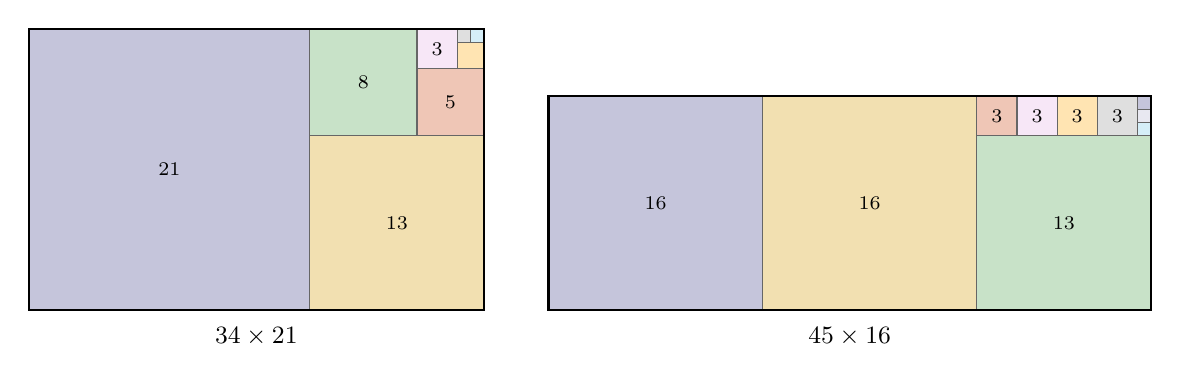
\begin{tikzpicture}
  \filldraw[fill=MidnightBlue!25,draw=black!60] (0.000,0.000) rectangle ++(3.570,3.570);
  \node[font=\scriptsize] at (1.785,1.785) {21};
  \filldraw[fill=Goldenrod!35,draw=black!60] (3.570,0.000) rectangle ++(2.210,2.210);
  \node[font=\scriptsize] at (4.675,1.105) {13};
  \filldraw[fill=ForestGreen!25,draw=black!60] (3.570,2.210) rectangle ++(1.360,1.360);
  \node[font=\scriptsize] at (4.250,2.890) {8};
  \filldraw[fill=BrickRed!20,draw=black!60] (4.930,2.210) rectangle ++(0.850,0.850);
  \node[font=\scriptsize] at (5.355,2.635) {5};
  \filldraw[fill=Plum!25,draw=black!60] (4.930,3.060) rectangle ++(0.510,0.510);
  \node[font=\scriptsize] at (5.185,3.315) {3};
  \filldraw[fill=Orange!30,draw=black!60] (5.440,3.060) rectangle ++(0.340,0.340);
  \filldraw[fill=gray!25,draw=black!60] (5.440,3.400) rectangle ++(0.170,0.170);
  \filldraw[fill=SkyBlue!35,draw=black!60] (5.610,3.400) rectangle ++(0.170,0.170);
  \draw[thick] (0,0) rectangle ++(5.780,3.570);
  \node[below,font=\small] at (2.890,-0.1) {$34\times21$};
  \filldraw[fill=MidnightBlue!25,draw=black!60] (6.600,0.000) rectangle ++(2.720,2.720);
  \node[font=\scriptsize] at (7.960,1.360) {16};
  \filldraw[fill=Goldenrod!35,draw=black!60] (9.320,0.000) rectangle ++(2.720,2.720);
  \node[font=\scriptsize] at (10.680,1.360) {16};
  \filldraw[fill=ForestGreen!25,draw=black!60] (12.040,0.000) rectangle ++(2.210,2.210);
  \node[font=\scriptsize] at (13.145,1.105) {13};
  \filldraw[fill=BrickRed!20,draw=black!60] (12.040,2.210) rectangle ++(0.510,0.510);
  \node[font=\scriptsize] at (12.295,2.465) {3};
  \filldraw[fill=Plum!25,draw=black!60] (12.550,2.210) rectangle ++(0.510,0.510);
  \node[font=\scriptsize] at (12.805,2.465) {3};
  \filldraw[fill=Orange!30,draw=black!60] (13.060,2.210) rectangle ++(0.510,0.510);
  \node[font=\scriptsize] at (13.315,2.465) {3};
  \filldraw[fill=gray!25,draw=black!60] (13.570,2.210) rectangle ++(0.510,0.510);
  \node[font=\scriptsize] at (13.825,2.465) {3};
  \filldraw[fill=SkyBlue!35,draw=black!60] (14.080,2.210) rectangle ++(0.170,0.170);
  \filldraw[fill=MidnightBlue!10,draw=black!60] (14.080,2.380) rectangle ++(0.170,0.170);
  \filldraw[fill=MidnightBlue!25,draw=black!60] (14.080,2.550) rectangle ++(0.170,0.170);
  \draw[thick] (6.6,0) rectangle ++(7.650,2.720);
  \node[below,font=\small] at (10.425,-0.1) {$45\times16$};
\end{tikzpicture}
